% ====================================================================
% ФАЙЛ: tasks/03_electrodynamics/oscillatory_circuit_part1.tex
% ТЕМА: КОЛЕБАТЕЛЬНЫЙ КОНТУР
% ПАЧКА 1: ВАРИАНТЫ 1–10
% ====================================================================

% === ЗАДАЧА 1 ===
% Тег: #ЭЛЕКТРОДИНАМИКА #КОЛЕБАНИЯ #КОЛЕБАТЕЛЬНЫЙ_КОНТУР #КИМ_13 #ВАРИАНТ_01
\begin{taskbasic}[code={\label{task:elem_osc_v1_n13}}]
Идеальный колебательный контур состоит из конденсатора ёмкостью $C$ и катушки индуктивностью $L$. Во сколько раз уменьшится период собственных электромагнитных колебаний в этом контуре, если его индуктивность уменьшить в 8 раз, а ёмкость уменьшить в 2 раза?

\kim{13}
\end{taskbasic}
\answer{4}

% === ЗАДАЧА 2 ===
% Тег: #ЭЛЕКТРОДИНАМИКА #КОЛЕБАНИЯ #КОЛЕБАТЕЛЬНЫЙ_КОНТУР #КИМ_13 #ВАРИАНТ_02
\begin{taskbasic}[code={\label{task:elem_osc_v2_n13}}]
Идеальный колебательный контур состоит из конденсатора ёмкостью $C$ и катушки индуктивностью $L$. Во сколько раз уменьшится частота собственных электромагнитных колебаний в этом контуре, если его индуктивность увеличить в 18 раз, а ёмкость уменьшить в 2 раза?

\kim{13}
\end{taskbasic}
\answer{3}

% === ЗАДАЧА 3 ===
% Тег: #ЭЛЕКТРОДИНАМИКА #КОЛЕБАНИЯ #КОЛЕБАТЕЛЬНЫЙ_КОНТУР #КИМ_14 #ВАРИАНТ_03
\begin{taskbasic}[code={\label{task:elem_osc_v3_n14}}]
В идеальном колебательном контуре, состоящем из конденсатора и катушки индуктивности, происходят свободные электромагнитные колебания. В таблице показано, как изменяется заряд на одной из пластин конденсатора в колебательном контуре с течением времени.

\nopagebreak\smallskip
\begin{center}
\small
\begin{tabular}{|l|c|c|c|c|c|c|c|c|c|c|}
\hline
$t$, $10^{-6}\text{ с}$ & 0 & 1 & 2 & 3 & 4 & 5 & 6 & 7 & 8 & 9 \\ \hline
$q$, $10^{-9}\text{ Кл}$ & 2 & 1,42 & 0 & --1,42 & --2 & --1,42 & 0 & 1,42 & 2 & 1,42 \\ \hline
\end{tabular}
\end{center}
\smallskip

Выберите все верные утверждения о процессе, происходящем в контуре.

1) В момент времени $t = 6\cdot 10^{-6}\text{ с}$ сила тока в контуре равна нулю.\\
2) Период колебаний энергии магнитного поля катушки равен $8\cdot 10^{-6}\text{ с}$.\\
3) В момент времени $t = 4\cdot 10^{-6}\text{ с}$ энергия электрического поля конденсатора максимальна.\\
4) В момент времени $t = 2\cdot 10^{-6}\text{ с}$ модуль силы тока в контуре максимален.\\
5) Частота электромагнитных колебаний в контуре равна $125\text{ кГц}$.

\kim{14}
\end{taskbasic}
\answer{345}

% === ЗАДАЧА 4 ===
% Тег: #ЭЛЕКТРОДИНАМИКА #КОЛЕБАНИЯ #КОЛЕБАТЕЛЬНЫЙ_КОНТУР #КИМ_14 #ВАРИАНТ_04
\begin{taskbasic}[code={\label{task:elem_osc_v4_n14}}]
В идеальном колебательном контуре, состоящем из конденсатора и катушки индуктивности, происходят свободные электромагнитные колебания. В таблице показано, как изменяется заряд на одной из пластин конденсатора в колебательном контуре с течением времени.

\nopagebreak\smallskip
\begin{center}
\small
\begin{tabular}{|l|c|c|c|c|c|c|c|c|c|c|}
\hline
$t$, $10^{-6}\text{ с}$ & 0 & 1 & 2 & 3 & 4 & 5 & 6 & 7 & 8 & 9 \\ \hline
$q$, $10^{-9}\text{ Кл}$ & 2 & 1,42 & 0 & --1,42 & --2 & --1,42 & 0 & 1,42 & 2 & 1,42 \\ \hline
\end{tabular}
\end{center}
\smallskip

Выберите все верные утверждения о процессе, происходящем в контуре.

1) В момент времени $t = 8\cdot 10^{-6}\text{ с}$ сила тока в контуре равна нулю.\\
2) Период электромагнитных колебаний в контуре равен $8\text{ мкс}$.\\
3) В момент времени $t = 4\cdot 10^{-6}\text{ с}$ энергия электрического поля конденсатора минимальна.\\
4) В момент времени $t = 2\cdot 10^{-6}\text{ с}$ модуль силы тока в контуре минимальный.\\
5) Частота электромагнитных колебаний в контуре равна $125\text{ кГц}$.

\kim{14}
\end{taskbasic}
\answer{23}

% === ЗАДАЧА 5 ===
% Тег: #ЭЛЕКТРОДИНАМИКА #КОЛЕБАНИЯ #КОЛЕБАТЕЛЬНЫЙ_КОНТУР #КИМ_15 #ВАРИАНТ_05
\begin{taskbasic}[code={\label{task:elem_osc_v5_n15}}]
Конденсатор идеального колебательного контура длительное время подключён к источнику постоянного напряжения. В момент $t = 0$ переключатель $K$ перевели из положения 1 в положение 2. Графики А и Б отражают изменение с течением времени физических величин, характеризующих свободные электромагнитные колебания, возникшие в контуре после этого ($T$ --- период колебаний).

\nopagebreak\smallskip
\begin{center}
\begin{tikzpicture}[scale=1.0, every node/.style={font=\footnotesize}]
    \draw[xstep=1, ystep=1, gray!30, thin] (0,0) grid (4,3);
    
    % График А
    \draw[ultra thick, brandPrimary] plot[domain=0:4, samples=100] (\x, {1.5 - 1.5*cos(\x*180)});
    
    \node[below left] at (0,0) {0};
    \node[below] at (4,0) {$T$};
    \node[below] at (2,0) {$t$};
\end{tikzpicture}
\qquad
\begin{tikzpicture}[scale=1.0, every node/.style={font=\footnotesize}]
    \draw[xstep=1, ystep=1, gray!30, thin] (0,0) grid (4,3);
    
    % График Б
    \draw[ultra thick, brandPrimary] plot[domain=0:4, samples=100] (\x, {1.5 + 1.5*cos(\x*90)});
    
    \node[below left] at (0,0) {0};
    \node[below] at (4,0) {$T$};
    \node[below] at (2,0) {$t$};
\end{tikzpicture}
\end{center}

Установите соответствие между графиками и физическими величинами, зависимость которых от времени эти графики могут изображать.

\smallskip
\begin{tabular}{p{0.45\textwidth}p{0.5\textwidth}}
\textbf{ГРАФИКИ} & \textbf{ФИЗИЧЕСКИЕ ВЕЛИЧИНЫ} \\
А) График А & 1) заряд правой обкладки конденсатора \\
Б) График Б & 2) энергия магнитного поля катушки \\
& 3) энергия электрического поля конденсатора \\
& 4) сила тока в катушке
\end{tabular}

\kim{15}
\end{taskbasic}
\answer{21}

% === ЗАДАЧА 6 ===
% Тег: #ЭЛЕКТРОДИНАМИКА #КОЛЕБАНИЯ #КОЛЕБАТЕЛЬНЫЙ_КОНТУР #КИМ_15 #ВАРИАНТ_06
\begin{taskbasic}[code={\label{task:elem_osc_v6_n15}}]
Конденсатор идеального колебательного контура длительное время подключён к источнику постоянного напряжения. В момент $t = 0$ переключатель $K$ перевели из положения 1 в положение 2. Графики А и Б отражают изменение с течением времени физических величин, характеризующих свободные электромагнитные колебания, возникшие в контуре после этого ($T$ --- период колебаний).

Установите соответствие между графиками и физическими величинами, зависимость которых от времени эти графики могут изображать.

\smallskip
\begin{tabular}{p{0.45\textwidth}p{0.5\textwidth}}
\textbf{ГРАФИКИ} & \textbf{ФИЗИЧЕСКИЕ ВЕЛИЧИНЫ} \\
А) График А & 1) заряд левой обкладки конденсатора \\
Б) График Б & 2) модуль напряжения на конденсаторе \\
& 3) энергия электрического поля конденсатора \\
& 4) сила тока в катушке
\end{tabular}

\kim{15}
\end{taskbasic}
\answer{34}

% === ЗАДАЧА 7 ===
% Тег: #ЭЛЕКТРОДИНАМИКА #КОЛЕБАНИЯ #КОЛЕБАТЕЛЬНЫЙ_КОНТУР #КИМ_14 #ВАРИАНТ_07
\begin{taskbasic}[code={\label{task:elem_osc_v7_n14}}]
В идеальном колебательном контуре, состоящем из конденсатора и катушки индуктивности, происходят свободные электромагнитные колебания. Изменение заряда на одной из обкладок конденсатора с течением времени показано в таблице.

\nopagebreak\smallskip
\begin{center}
\small
\begin{tabular}{|l|c|c|c|c|c|c|c|c|c|c|}
\hline
$t$, $10^{-6}\text{ с}$ & 0 & 1 & 2 & 3 & 4 & 5 & 6 & 7 & 8 & 9 \\ \hline
$q$, $10^{-9}\text{ Кл}$ & 1 & 0,71 & 0 & --0,71 & --1 & --0,71 & 0 & 0,71 & 1 & 0,71 \\ \hline
\end{tabular}
\end{center}
\smallskip

Выберите все верные утверждения о процессах, происходящих в контуре.

1) Период колебаний равен $4\text{ мкс}$.\\
2) Частота колебаний равна $125\text{ кГц}$.\\
3) В момент времени $t = 2\cdot 10^{-6}\text{ с}$ модуль силы тока в катушке индуктивности максимален.\\
4) В момент времени $t = 8\cdot 10^{-6}\text{ с}$ энергия магнитного поля катушки индуктивности максимальна.\\
5) В момент времени $t = 6\cdot 10^{-6}\text{ с}$ модуль напряжения на конденсаторе минимален.

\kim{14}
\end{taskbasic}
\answer{235}

% === ЗАДАЧА 8 ===
% Тег: #ЭЛЕКТРОДИНАМИКА #КОЛЕБАНИЯ #КОЛЕБАТЕЛЬНЫЙ_КОНТУР #КИМ_14 #ВАРИАНТ_08
\begin{taskbasic}[code={\label{task:elem_osc_v8_n14}}]
В идеальном колебательном контуре, состоящем из конденсатора и катушки индуктивности, происходят свободные электромагнитные колебания. Изменение заряда одной из обкладок конденсатора с течением времени показано в таблице.

\nopagebreak\smallskip
\begin{center}
\small
\begin{tabular}{|l|c|c|c|c|c|c|c|c|c|c|}
\hline
$t$, $10^{-6}\text{ с}$ & 0 & 1 & 2 & 3 & 4 & 5 & 6 & 7 & 8 & 9 \\ \hline
$q$, $10^{-9}\text{ Кл}$ & 1 & 0,71 & 0 & --0,71 & --1 & --0,71 & 0 & 0,71 & 1 & 0,71 \\ \hline
\end{tabular}
\end{center}
\smallskip

Выберите все верные утверждения о процессах, происходящих в контуре.

1) Период колебаний равен $8\cdot 10^{-6}\text{ с}$.\\
2) Частота колебаний равна $250\text{ кГц}$.\\
3) В момент времени $t = 2\cdot 10^{-6}\text{ с}$ сила тока в катушке индуктивности равна нулю.\\
4) В момент времени $t = 8\cdot 10^{-6}\text{ с}$ энергия магнитного поля катушки индуктивности минимальна.\\
5) В момент времени $t = 4\cdot 10^{-6}\text{ с}$ энергия электрического поля конденсатора минимальна.

\kim{14}
\end{taskbasic}
\answer{14}

% === ЗАДАЧА 9 ===
% Тег: #ЭЛЕКТРОДИНАМИКА #КОЛЕБАНИЯ #КОЛЕБАТЕЛЬНЫЙ_КОНТУР #КИМ_23 #ВАРИАНТ_01
\begin{taskbasic}[code={\label{task:elem_osc_v1_n23}}]
В идеальном колебательном контуре напряжение между обкладками конденсатора меняется по закону $U_C = 0{,}2 \cdot \sin(5000t + \pi)$. Максимальное значение силы тока в контуре $I_{\max} = 2\text{ мА}$. Определите электроёмкость конденсатора. Ответ выразите в фарадах (Ф).

\nopagebreak\smallskip
\begin{center}
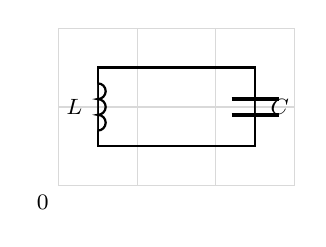
\begin{tikzpicture}[scale=1.0, every node/.style={font=\footnotesize}]
    \draw[xstep=1, ystep=1, gray!30, thin] (0,0) grid (3,2);
    
    \draw[thick, black] (0.5,0.5) -- (0.5,1.5) -- (2.5,1.5) -- (2.5,0.5) -- cycle;
    
    % Катушка L (слева)
    \fill[white] (0.5,0.7) rectangle (0.5,1.3);
    \draw[thick, black] (0.5,0.5) -- (0.5,0.7);
    \draw[thick, black] (0.5,0.7) arc (-90:90:0.1) arc (-90:90:0.1) arc (-90:90:0.1);
    \draw[thick, black] (0.5,1.3) -- (0.5,1.5);
    \node[left=2pt] at (0.5,1.0) {$L$};
    
    % Конденсатор C (справа)
    \fill[white] (2.5,0.8) rectangle (2.5,1.2);
    \draw[thick, black] (2.5,0.5) -- (2.5,0.9);
    \draw[ultra thick, black] (2.2,0.9) -- (2.8,0.9);
    \draw[ultra thick, black] (2.2,1.1) -- (2.8,1.1);
    \draw[thick, black] (2.5,1.1) -- (2.5,1.5);
    \node[right=2pt] at (2.5,1.0) {$C$};
    
    \node[below left] at (0,0) {0};
\end{tikzpicture}
\end{center}

\kim{23}
\end{taskbasic}
\answer{$2\cdot 10^{-6}$}

% === ЗАДАЧА 10 ===
% Тег: #ЭЛЕКТРОДИНАМИКА #КОЛЕБАНИЯ #КОЛЕБАТЕЛЬНЫЙ_КОНТУР #КИМ_23 #ВАРИАНТ_02
\begin{taskbasic}[code={\label{task:elem_osc_v2_n23}}]
В идеальном колебательном контуре напряжение между обкладками конденсатора меняется по закону $U_C = 20 \cdot \sin(5000t + \pi)$. Максимальное значение силы тока в контуре $I_{\max} = 0{,}2\text{ А}$. Определите индуктивность катушки. Ответ выразите в генри (Гн).

\kim{23}
\end{taskbasic}
\answer{0,02}

% ====================================================================
% ФАЙЛ: tasks/03_electrodynamics/oscillatory_circuit_part2.tex
% ТЕМА: КОЛЕБАТЕЛЬНЫЙ КОНТУР
% ПАЧКА 2: ВАРИАНТЫ 11–20
% ====================================================================

% === ЗАДАЧА 1 ===
% Тег: #ЭЛЕКТРОДИНАМИКА #КОЛЕБАНИЯ #КОЛЕБАТЕЛЬНЫЙ_КОНТУР #КИМ_13 #ВАРИАНТ_11
\begin{taskbasic}[code={\label{task:elem_osc_v11_n13}}]
Идеальный колебательный контур состоит из конденсатора ёмкостью $C$ и катушки индуктивностью $L$. Во сколько раз увеличится период собственных электромагнитных колебаний в этом контуре, если его индуктивность увеличить в 2 раза, а ёмкость увеличить в 8 раз?

\kim{13}
\end{taskbasic}
\answer{4}

% === ЗАДАЧА 2 ===
% Тег: #ЭЛЕКТРОДИНАМИКА #КОЛЕБАНИЯ #КОЛЕБАТЕЛЬНЫЙ_КОНТУР #КИМ_13 #ВАРИАНТ_12
\begin{taskbasic}[code={\label{task:elem_osc_v12_n13}}]
Идеальный колебательный контур состоит из конденсатора ёмкостью $C$ и катушки индуктивностью $L$. Во сколько раз увеличится частота собственных электромагнитных колебаний в этом контуре, если его индуктивность увеличить в 2 раза, а ёмкость уменьшить в 18 раз?

\kim{13}
\end{taskbasic}
\answer{3}

% === ЗАДАЧА 3 ===
% Тег: #ЭЛЕКТРОДИНАМИКА #КОЛЕБАНИЯ #КОЛЕБАТЕЛЬНЫЙ_КОНТУР #КИМ_14 #ВАРИАНТ_17
\begin{taskbasic}[code={\label{task:elem_osc_v17_n14}}]
В идеальном колебательном контуре, состоящем из конденсатора и катушки индуктивности, происходят свободные электромагнитные колебания. В таблице показано, как изменяется заряд на одной из пластин конденсатора с течением времени.

\nopagebreak\smallskip
\begin{center}
\small
\begin{tabular}{|l|c|c|c|c|c|c|c|c|c|c|}
\hline
$t$, $10^{-6}\text{ с}$ & 0 & 1 & 2 & 3 & 4 & 5 & 6 & 7 & 8 & 9 \\ \hline
$q$, $10^{-9}\text{ Кл}$ & 4 & 2,83 & 0 & --2,83 & --4 & --2,83 & 0 & 2,83 & 4 & 2,83 \\ \hline
\end{tabular}
\end{center}
\smallskip

Выберите все верные утверждения о процессе, происходящем в контуре.

1) В момент времени $t = 2\cdot 10^{-6}\text{ с}$ сила тока в контуре максимальна.\\
2) Период электромагнитных колебаний в контуре равен $4\text{ мкс}$.\\
3) В момент времени $t = 4\cdot 10^{-6}\text{ с}$ энергия электрического поля конденсатора минимальна.\\
4) В момент времени $t = 6\cdot 10^{-6}\text{ с}$ энергия магнитного поля катушки максимальна.\\
5) Частота электромагнитных колебаний в контуре равна $125\text{ кГц}$.

\kim{14}
\end{taskbasic}
\answer{145}

% === ЗАДАЧА 4 ===
% Тег: #ЭЛЕКТРОДИНАМИКА #КОЛЕБАНИЯ #КОЛЕБАТЕЛЬНЫЙ_КОНТУР #КИМ_14 #ВАРИАНТ_18
\begin{taskbasic}[code={\label{task:elem_osc_v18_n14}}]
В идеальном колебательном контуре, состоящем из конденсатора и катушки индуктивности, происходят свободные электромагнитные колебания. В таблице показано, как изменяется заряд одной из обкладок конденсатора с течением времени.

\nopagebreak\smallskip
\begin{center}
\small
\begin{tabular}{|l|c|c|c|c|c|c|c|c|c|c|}
\hline
$t$, $10^{-6}\text{ с}$ & 0 & 1 & 2 & 3 & 4 & 5 & 6 & 7 & 8 & 9 \\ \hline
$q$, $10^{-9}\text{ Кл}$ & 4 & 2,83 & 0 & --2,83 & --4 & --2,83 & 0 & 2,83 & 4 & 2,83 \\ \hline
\end{tabular}
\end{center}
\smallskip

Выберите все верные утверждения о процессе, происходящем в контуре.

1) В момент времени $t = 2\cdot 10^{-6}\text{ с}$ сила тока в контуре равна нулю.\\
2) Период колебаний равен $4\cdot 10^{-6}\text{ с}$.\\
3) В момент времени $t = 4\cdot 10^{-6}\text{ с}$ энергия электрического поля конденсатора максимальна.\\
4) В момент времени $t = 6\cdot 10^{-6}\text{ с}$ энергия магнитного поля катушки равна нулю.\\
5) В момент времени $t = 2\cdot 10^{-6}\text{ с}$ модуль силы тока в контуре максимален.

\kim{14}
\end{taskbasic}
\answer{35}

% === ЗАДАЧА 5 ===
% Тег: #ЭЛЕКТРОДИНАМИКА #КОЛЕБАНИЯ #КОЛЕБАТЕЛЬНЫЙ_КОНТУР #КИМ_15 #ВАРИАНТ_19
\begin{taskbasic}[code={\label{task:elem_osc_v19_n15}}]
Конденсатор идеального колебательного контура длительное время подключён к источнику постоянного напряжения. В момент $t = 0$ переключатель $K$ перевели из положения 1 в положение 2. Графики А и Б отражают изменение с течением времени физических величин, характеризующих свободные электромагнитные колебания, возникшие в контуре после этого ($T$ --- период колебаний).

\nopagebreak\smallskip
\begin{center}
\begin{tikzpicture}[scale=1.0, every node/.style={font=\footnotesize}]
    \draw[xstep=1, ystep=1, gray!30, thin] (0,0) grid (4,3);
    
    % График А
    \draw[ultra thick, brandPrimary] plot[domain=0:4, samples=100] (\x, {1.5 + 1.5*cos(\x*180)});
    
    \node[below left] at (0,0) {0};
    \node[below] at (4,0) {$T$};
    \node[below] at (2,0) {$t$};
\end{tikzpicture}
\qquad
\begin{tikzpicture}[scale=1.0, every node/.style={font=\footnotesize}]
    \draw[xstep=1, ystep=1, gray!30, thin] (0,0) grid (4,3);
    
    % График Б
    \draw[ultra thick, brandPrimary] plot[domain=0:4, samples=100] (\x, {1.5 - 1.5*sin(\x*90)});
    
    \node[below left] at (0,0) {0};
    \node[below] at (4,0) {$T$};
    \node[below] at (2,0) {$t$};
\end{tikzpicture}
\end{center}

Установите соответствие между графиками и физическими величинами, зависимость которых от времени эти графики могут изображать.

\smallskip
\begin{tabular}{p{0.45\textwidth}p{0.5\textwidth}}
\textbf{ГРАФИКИ} & \textbf{ФИЗИЧЕСКИЕ ВЕЛИЧИНЫ} \\
А) График А & 1) заряд правой обкладки конденсатора \\
Б) График Б & 2) сила тока в катушке \\
& 3) энергия электрического поля конденсатора \\
& 4) энергия магнитного поля катушки
\end{tabular}

\kim{15}
\end{taskbasic}
\answer{32}

% === ЗАДАЧА 6 ===
% Тег: #ЭЛЕКТРОДИНАМИКА #КОЛЕБАНИЯ #КОЛЕБАТЕЛЬНЫЙ_КОНТУР #КИМ_15 #ВАРИАНТ_20
\begin{taskbasic}[code={\label{task:elem_osc_v20_n15}}]
Конденсатор идеального колебательного контура длительное время подключён к источнику постоянного напряжения. В момент $t = 0$ переключатель $K$ перевели из положения 1 в положение 2. Графики А и Б отражают изменение с течением времени физических величин, характеризующих свободные электромагнитные колебания в контуре после этого ($T$ --- период колебаний).

Установите соответствие между графиками и физическими величинами, зависимость которых от времени эти графики могут изображать.

\smallskip
\begin{tabular}{p{0.45\textwidth}p{0.5\textwidth}}
\textbf{ГРАФИКИ} & \textbf{ФИЗИЧЕСКИЕ ВЕЛИЧИНЫ} \\
А) График А & 1) заряд правой обкладки конденсатора \\
Б) График Б & 2) сила тока в катушке \\
& 3) энергия электрического поля конденсатора \\
& 4) энергия магнитного поля катушки
\end{tabular}

\kim{15}
\end{taskbasic}
\answer{41}

% ====================================================================
% ФАЙЛ: tasks/03_electrodynamics/oscillatory_circuit_part3.tex
% ТЕМА: КОЛЕБАТЕЛЬНЫЙ КОНТУР
% ПАЧКА 3: ВАРИАНТЫ 21–30
% ====================================================================

% === ЗАДАЧА 1 ===
% Тег: #ЭЛЕКТРОДИНАМИКА #КОЛЕБАНИЯ #КОЛЕБАТЕЛЬНЫЙ_КОНТУР #КИМ_13 #ВАРИАНТ_21
\begin{taskbasic}[code={\label{task:elem_osc_v21_n13}}]
Идеальный колебательный контур состоит из конденсатора ёмкостью $C$ и катушки индуктивностью $L$. Во сколько раз уменьшится период собственных электромагнитных колебаний в этом контуре, если его индуктивность уменьшить в 8 раз, а ёмкость уменьшить в 2 раза?

\kim{13}
\end{taskbasic}
\answer{4}

% === ЗАДАЧА 2 ===
% Тег: #ЭЛЕКТРОДИНАМИКА #КОЛЕБАНИЯ #КОЛЕБАТЕЛЬНЫЙ_КОНТУР #КИМ_13 #ВАРИАНТ_22
\begin{taskbasic}[code={\label{task:elem_osc_v22_n13}}]
Идеальный колебательный контур состоит из конденсатора ёмкостью $C$ и катушки индуктивностью $L$. Во сколько раз уменьшится частота собственных электромагнитных колебаний в этом контуре, если его индуктивность увеличить в 18 раз, а ёмкость уменьшить в 2 раза?

\kim{13}
\end{taskbasic}
\answer{3}

% === ЗАДАЧА 3 ===
% Тег: #ЭЛЕКТРОДИНАМИКА #КОЛЕБАНИЯ #КОЛЕБАТЕЛЬНЫЙ_КОНТУР #КИМ_14 #ВАРИАНТ_25
\begin{taskbasic}[code={\label{task:elem_osc_v25_n14}}]
В идеальном колебательном контуре, состоящем из конденсатора и катушки индуктивности, происходят свободные электромагнитные колебания. В таблице показано, как изменяется заряд одной из обкладок конденсатора с течением времени.

\nopagebreak\smallskip
\begin{center}
\small
\begin{tabular}{|l|c|c|c|c|c|c|c|c|c|c|}
\hline
$t$, $10^{-6}\text{ с}$ & 0 & 1 & 2 & 3 & 4 & 5 & 6 & 7 & 8 & 9 \\ \hline
$q$, $10^{-9}\text{ Кл}$ & 3 & 2,12 & 0 & --2,12 & --3 & --2,12 & 0 & 2,12 & 3 & 2,12 \\ \hline
\end{tabular}
\end{center}
\smallskip

Выберите все верные утверждения о процессе, происходящем в контуре.

1) В момент времени $t = 2\cdot 10^{-6}\text{ с}$ модуль силы тока в контуре максимален.\\
2) Период электромагнитных колебаний в контуре равен $4\text{ мкс}$.\\
3) В момент времени $t = 4\cdot 10^{-6}\text{ с}$ энергия электрического поля конденсатора максимальна.\\
4) В момент времени $t = 6\cdot 10^{-6}\text{ с}$ энергия магнитного поля катушки минимальна.\\
5) Частота электромагнитных колебаний в контуре равна $250\text{ кГц}$.

\kim{14}
\end{taskbasic}
\answer{13}

% === ЗАДАЧА 4 ===
% Тег: #ЭЛЕКТРОДИНАМИКА #КОЛЕБАНИЯ #КОЛЕБАТЕЛЬНЫЙ_КОНТУР #КИМ_14 #ВАРИАНТ_26
\begin{taskbasic}[code={\label{task:elem_osc_v26_n14}}]
В идеальном колебательном контуре, состоящем из конденсатора и катушки индуктивности, происходят свободные электромагнитные колебания. В таблице показано, как изменяется заряд на одной из пластин конденсатора с течением времени.

\nopagebreak\smallskip
\begin{center}
\small
\begin{tabular}{|l|c|c|c|c|c|c|c|c|c|c|}
\hline
$t$, $10^{-6}\text{ с}$ & 0 & 1 & 2 & 3 & 4 & 5 & 6 & 7 & 8 & 9 \\ \hline
$q$, $10^{-9}\text{ Кл}$ & 3 & 2,12 & 0 & --2,12 & --3 & --2,12 & 0 & 2,12 & 3 & 2,12 \\ \hline
\end{tabular}
\end{center}
\smallskip

Выберите все верные утверждения о процессе, происходящем в контуре.

1) Период электромагнитных колебаний в контуре равен $8\text{ мкс}$.\\
2) В момент времени $t = 4\cdot 10^{-6}\text{ с}$ сила тока в контуре максимальна.\\
3) В момент времени $t = 2\cdot 10^{-6}\text{ с}$ энергия электрического поля конденсатора максимальна.\\
4) В момент времени $t = 2\cdot 10^{-6}\text{ с}$ энергия магнитного поля катушки максимальна.\\
5) Частота электромагнитных колебаний в контуре равна $125\text{ кГц}$.

\kim{14}
\end{taskbasic}
\answer{145}

% === ЗАДАЧА 5 ===
% Тег: #ЭЛЕКТРОДИНАМИКА #КОЛЕБАНИЯ #КОЛЕБАТЕЛЬНЫЙ_КОНТУР #КИМ_23 #ВАРИАНТ_21
\begin{taskbasic}[code={\label{task:elem_osc_v21_n23}}]
В идеальном колебательном контуре напряжение между обкладками конденсатора меняется по закону $U_C = 0{,}2 \cdot \sin(5000t + \pi)$. Максимальное значение силы тока в контуре $I_{\max} = 2\text{ мА}$. Определите электроёмкость конденсатора. Ответ выразите в фарадах (Ф).

\kim{23}
\end{taskbasic}
\answer{$2\cdot 10^{-6}$}

% === ЗАДАЧА 6 ===
% Тег: #ЭЛЕКТРОДИНАМИКА #КОЛЕБАНИЯ #КОЛЕБАТЕЛЬНЫЙ_КОНТУР #КИМ_22 #ВАРИАНТ_22
\begin{taskbasic}[code={\label{task:elem_osc_v22_n23}}]
В идеальном колебательном контуре напряжение между обкладками конденсатора меняется по закону $U_C = 20 \cdot \sin(5000t + \pi)$. Максимальное значение силы тока в контуре $I_{\max} = 0{,}2\text{ А}$. Определите индуктивность катушки. Ответ выразите в генри (Гн).

\kim{23}
\end{taskbasic}
\answer{0,02}

\begin{center}
\begin{tikzpicture}[scale=1.1, font=\small, >=Stealth]

  % --- Координатные оси ---
  % Ось x (направление распространения)
  \draw[thick, ->] (-0.5, 0, 0) -- (9.5, 0, 0) node[right, font=\large\itshape] {$x$};
  % Ось y (электрическое поле E)
  \draw[thick, ->] (0, -2.2, 0) -- (0, 2.4, 0) node[above, font=\large\bfseries] {$\mathbf{E}$};
  
  % Ось z (магнитное поле B)
  \draw[thick, ->] (0, 0, -0.5) -- (0, 0, 3.2);

  % --- Вектор скорости волны c ---
  \draw[ultra thick, red, ->] (-1.2, 0, 0) -- (-0.2, 0, 0) 
    node[midway, above left, font=\large\bfseries, color=red] {$\mathbf{c}$};

  % --- Параметры волны ---
  \def\waveL{4.0} % Длина волны
  \def\ampY{1.8}  % Амплитуда по Y (E)
  \def\ampZ{2.0}  % Амплитуда по Z (B)

  % --- РИСОВАНИЕ 3D ЭЛЕКТРОМАГНИТНОЙ ВОЛНЫ ---

  % 1. Составляющая E (колебания в плоскости xy, желтая заливка)
  % Заливка полуволн E
  \fill[orange!25, opacity=0.7] 
    plot[domain=0:\waveL, samples=60] (\x, {\ampY*sin(\x*360/\waveL)}, 0) -- (0,0,0);
  \fill[orange!25, opacity=0.7] 
    plot[domain=\waveL:2*\waveL, samples=60] (\x, {\ampY*sin(\x*360/\waveL)}, 0) -- (\waveL,0,0);

  % Огибающая E
  \draw[very thick, orange!80!black] 
    plot[domain=0:2*\waveL, samples=100] (\x, {\ampY*sin(\x*360/\waveL)}, 0);

  % Векторы напряженности E (стрелки)
  \foreach \x in {0.4, 0.8, 1.2, 1.6, 2.0} {
    \draw[thick, orange!80!black, ->] (\x, 0, 0) -- (\x, {\ampY*sin(\x*360/\waveL)}, 0);
  }
  \foreach \x in {2.4, 2.8, 3.2, 3.6} {
    \draw[thick, orange!80!black, ->] (\x, 0, 0) -- (\x, {\ampY*sin(\x*360/\waveL)}, 0);
  }
  \foreach \x in {4.4, 4.8, 5.2, 5.6, 6.0} {
    \draw[thick, orange!80!black, ->] (\x, 0, 0) -- (\x, {\ampY*sin(\x*360/\waveL)}, 0);
  }
  \foreach \x in {6.4, 6.8, 7.2, 7.6} {
    \draw[thick, orange!80!black, ->] (\x, 0, 0) -- (\x, {\ampY*sin(\x*360/\waveL)}, 0);
  }


  % 2. Составляющая B (колебания в плоскости xz, серо-голубая заливка)
  % Заливка полуволн B
  \fill[cyan!20!gray!30, opacity=0.75] 
    plot[domain=0:\waveL, samples=60] (\x, 0, {\ampZ*sin(\x*360/\waveL)}) -- (0,0,0);
  \fill[cyan!20!gray!30, opacity=0.75] 
    plot[domain=\waveL:2*\waveL, samples=60] (\x, 0, {\ampZ*sin(\x*360/\waveL)}) -- (\waveL,0,0);

  % Огибающая B
  \draw[very thick, cyan!40!black] 
    plot[domain=0:2*\waveL, samples=100] (\x, 0, {\ampZ*sin(\x*360/\waveL)});

  % Векторы индукции B (стрелки)
  \foreach \x in {0.4, 0.8, 1.2, 1.6, 2.0} {
    \draw[thick, cyan!40!black, ->] (\x, 0, 0) -- (\x, 0, {\ampZ*sin(\x*360/\waveL)});
  }
  \foreach \x in {2.4, 2.8, 3.2, 3.6} {
    \draw[thick, cyan!40!black, ->] (\x, 0, 0) -- (\x, 0, {\ampZ*sin(\x*360/\waveL)});
  }
  \foreach \x in {4.4, 4.8, 5.2, 5.6, 6.0} {
    \draw[thick, cyan!40!black, ->] (\x, 0, 0) -- (\x, 0, {\ampZ*sin(\x*360/\waveL)});
  }
  \foreach \x in {6.4, 6.8, 7.2, 7.6} {
    \draw[thick, cyan!40!black, ->] (\x, 0, 0) -- (\x, 0, {\ampZ*sin(\x*360/\waveL)});
  }

  % Подпись вектора B
  \node[below left, font=\large\bfseries] at (0.6, 0, 1.8) {$\mathbf{B}$};

\end{tikzpicture}
\end{center}